Las \textbf{criptomonedas} son monedas digitales que utilizan tecnología 
criptográfica para asegurar y verificar las transacciones y para controlar 
la creación de nuevas unidades de la moneda. Las criptomonedas funcionan en una 
red descentralizada, lo que significa que no están controladas por ningún 
gobierno, banco central o entidad financiera.\\
\hfill \break
Cada criptomoneda tiene su propia \textbf{red de blockchain} (Figura \ref*{fig:redes}), 
que es un registro público descentralizado que registra todas las transacciones 
de la moneda. La blockchain es una base de datos distribuida que contiene 
todas las transacciones realizadas con la moneda desde su creación, y se 
utiliza para verificar y validar las transacciones y para asegurar que no 
se puedan crear unidades adicionales de la moneda sin cumplir ciertas 
condiciones.\\
\hfill \break
\begin{figure}[htb!]
    \caption{Las redes más populares según Metamask}
    \label{fig:redes}
    \centering
    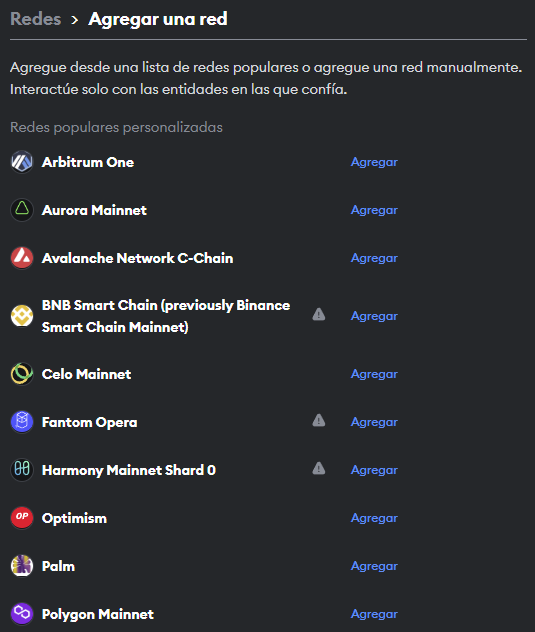
\includegraphics[scale=0.75]{./Ilustraciones/redes.png}\\
    \textbf{Fuente:} Cuenta personal de Metamask al querer agregar una nueva red a día 04/05/2023
\end{figure}
\hfill \break
Las \textbf{transacciones} en una criptomoneda se realizan de forma peer-to-peer (entre 
pares) y se validan a través de un proceso llamado \textbf{minería}. Esta es 
un proceso mediante el cual los usuarios de la red utilizan su poder
de cómputo para resolver problemas matemáticos complejos y validar las 
transacciones en la blockchain. Los usuarios que realizan esta tarea reciben 
recompensas en forma de nuevas unidades de la criptomoneda.\\
\hfill \break
Las criptomonedas se pueden comprar y vender en plataformas de intercambio de 
criptomonedas, y su valor depende de la oferta y la demanda del mercado.\\ 
\hfill \break
Ofrecen varias ventajas, como la descentralización, la transparencia, la 
seguridad y la privacidad, pero también presentan algunos desafíos, como la 
volatilidad del valor y la falta de regulación.\\
\hfill \break
En resumen, las criptomonedas son monedas digitales que utilizan tecnología 
criptográfica y una red descentralizada para asegurar y verificar las 
transacciones. Las criptomonedas se pueden comprar y vender en plataformas de 
intercambio, y su valor depende de la oferta y la demanda del mercado. Las 
criptomonedas como todo en la vida, tiene sus ventajas y sus riesgos.\\